\chapter{Perkembangan Reproduktif dan Kendali Pembungaan}\label{ch:b2:plant-flowering}

Seorang penanam krisan dapat membuat sebuah rumah kaca berbunga pada
Natal atau pada Paskah dengan menyalakan lampunya; gandum musim dingin
yang ditanam pada musim semi tidak pernah berbunga sama sekali, karena
ia belum kedinginan; sebatang kokelbur yang telah melihat satu malam
yang lebih panjang daripada panjang kritisnya terpancang untuk berbunga,
apa pun yang terjadi sesudahnya. Sebatang tumbuhan tidak memiliki
kalender, tetapi ia memiliki jam, termometer, dan pengukur cahaya, dan
ia memutuskan sekali setahun, atas bukti itu, untuk mengubah sebuah
\omterm{def:b2:plant-meristems:meristem}{meristem} yang selama ini membuat daun menjadi \omterm{def:b2:plant-meristems:meristem}{meristem} yang akan membuat
sekuntum \omterm{def:b2:angiosperm-reproduction:flower}{bunga}. Bab ini mengikuti keputusan itu dari daun yang mengukur
malamnya sampai ke \omterm{def:b2:plant-meristems:meristem}{meristem} yang mengganti programnya, lalu pembangunan
\omterm{def:b2:angiosperm-reproduction:flower}{bunganya} oleh sebuah sandi gen, dan peralihan sebaliknya pada ujung
daurnya yang lain: \omterm{def:b2:angiosperm-reproduction:seed}{biji} yang tidak mau berkecambah sampai ia diberi tahu
musimnya tepat.

\section{Peralihan menuju pembungaan}

\begin{definition}[Peralihan bunga dan pengimbasannya]\label{def:b2:plant-flowering:transition}
\index{peralihan bunga}\index{pengimbasan bunga}\index{meristem perbungaan}
Sebuah \omterm{def:b2:plant-meristems:meristem}{meristem apikal pucuk} yang vegetatif membuat daun dengan sebuah
tunas pada tiap ketiaknya, tanpa batas. Pada \emph{peralihan \omterm{def:b2:angiosperm-reproduction:flower}{bunga}}nya
ia menjadi sebuah \emph{\omterm{def:b2:plant-meristems:meristem}{meristem} perbungaan}, yang membuat braktea dan,
pada ketiaknya, \emph{\omterm{def:b2:plant-meristems:meristem}{meristem} \omterm{def:b2:angiosperm-reproduction:flower}{bunga}}, yang masing-masing bersifat
tertentu: ia membuat daun kelopak, daun mahkota, \omterm{def:b2:angiosperm-reproduction:flower}{benang sari}, dan \omterm{def:b2:angiosperm-reproduction:flower}{daun
buah} lalu berhenti. Perubahannya dipicu \emph{pengimbasan \omterm{def:b2:angiosperm-reproduction:flower}{bunga}} ---
sebuah isyarat, yang tiba dari daunnya atau muncul di dalam fisiologi
tumbuhannya sendiri, yang menyalakan gen jati diri \omterm{def:b2:plant-meristems:meristem}{meristemnya}.
Tumbuhan setahun berbunga sekali lalu mati; tumbuhan tahunan berbunga
tiap tahun dari sebagian \omterm{def:b2:plant-meristems:meristem}{meristemnya} dan menjaga sebagian lainnya tetap
vegetatif. Waktunya memutuskan apakah \omterm{def:b2:plant-life-cycles:heterospory}{serbuk sari} akan berjumpa dengan
\omterm{def:b2:plant-life-cycles:heterospory}{serbuk sari}, apakah \omterm{def:b2:angiosperm-reproduction:seed}{bijinya} masak sebelum embun beku, dan apakah \omterm{def:b2:angiosperm-reproduction:flower}{bunganya} membuka
ketika penyerbuknya terbang: ia berada di bawah seleksi yang kuat, dan
tumbuhan telah mengembangkan beberapa cara membaca musimnya.
\end{definition}

\begin{proposition}[Fotoperiodisme: tumbuhannya mengukur malamnya]\label{prop:b2:plant-flowering:photoperiod}
\index{fotoperiodisme}\index{tumbuhan hari pendek}%
\index{tumbuhan hari panjang}\index{fitokrom}
Banyak tumbuhan berbunga sebagai tanggapan terhadap panjang harinya.
\emph{\omterm{prop:b2:plant-flowering:photoperiod}{Tumbuhan hari pendek}} (krisan, kedelai, padi, kokelbur) berbunga
ketika harinya lebih pendek daripada sebuah panjang kritis --- pada
musim gugur atau musim semi; \emph{\omterm{prop:b2:plant-flowering:photoperiod}{tumbuhan hari panjang}} (bayam,
gandum, semanggi, \emph{Arabidopsis}) berbunga ketika harinya lebih
panjang --- pada awal musim panas; tumbuhan \emph{netral hari} (tomat,
jagung) berbunga ketika mereka sudah cukup besar. Yang sesungguhnya
diukur tumbuhannya adalah panjang \emph{malam} yang tak terputus:
\omterm{prop:b2:plant-flowering:photoperiod}{tumbuhan hari pendek} adalah tumbuhan malam panjang, dan sekilas cahaya
di tengah malam yang panjang meniadakan pengaruhnya, sedangkan sebuah
masa gelap di tengah hari yang panjang tidak. Pengukurannya dilakukan
di dalam \emph{daunnya}, oleh pigmen \emph{fitokrom} --- sebuah protein
yang berganti antara bentuk penyerap merah dan bentuk penyerap
merah-jauh tiap foton yang ditangkapnya, sehingga keadaannya merekam
cahayanya --- yang dibaca terhadap sebuah \emph{jam sirkadia} dalam
diri yang berperiode kira-kira dua puluh empat jam: pembungaannya
dipicu ketika cahayanya berimpit dengan sebuah fase tertentu jamnya,
dan hal itu hanya terjadi pada panjang hari yang tepat.
\end{proposition}
\begin{proof}[Bukti eksperimental]
Garner dan Allard (1920) mendapati bahwa sebuah mutan tembakau hanya
berbunga pada hari pendek sebuah rumah kaca musim dingin, dan bahwa
kedelai yang ditanam pada selang waktu sepanjang musim panas semuanya
berbunga bersama-sama pada bulan September: panjang harinya, bukan umur
maupun suhunya, yang menetapkan tanggalnya. Hamner dan Bonner (1938)
menunjukkan dengan kokelbur bahwa satu malam panjang sudah cukup, bahwa
semenit cahaya di tengah malamnya meniadakan pengaruhnya, dan bahwa
memendekkan harinya tanpa mengubah malamnya tidak mengimbas. Borthwick
dan Hendricks (1952) mendapati bahwa cahaya yang paling berdaya guna
adalah merah dan bahwa cahaya merah-jauh yang diberikan segera sesudah
merah meniadakannya --- tanda khas fitokrom, yang diisolasi pada 1959.
Mencangkokkan satu daun yang terimbas pada sebatang tumbuhan yang tak
terimbas membuat seluruh tumbuhannya berbunga: daunnya mengekspor
sebuah isyarat.
\end{proof}

\begin{omfigure}
\begin{tikzpicture}[every node/.style={font=\scriptsize}]
  \foreach \y/\lab/\res in {3.6/{hari panjang, malam pendek}/{tak berbunga}, 2.7/{hari pendek, malam panjang}/{berbunga}, 1.8/{malam panjang yang disela sekilas cahaya}/{tak berbunga}, 0.9/{hari panjang yang disela gelap}/{tak berbunga}} {
    \node[anchor=east, align=right] at (-0.2,\y) {\lab};
    \node[anchor=west, omThm] at (8.6,\y) {\res};
  }
  % bars: 24 h = 8 cm; light yellow, dark grey
  \fill[omExo!30] (0,3.4) rectangle (8,3.8); \fill[yellow!50!orange!40] (0,3.4) rectangle (5.4,3.8);
  \fill[omExo!30] (0,2.5) rectangle (8,2.9); \fill[yellow!50!orange!40] (0,2.5) rectangle (3.0,2.9);
  \fill[omExo!30] (0,1.6) rectangle (8,2.0); \fill[yellow!50!orange!40] (0,1.6) rectangle (3.0,2.0); \fill[yellow!50!orange!40] (5.4,1.6) rectangle (5.55,2.0);
  \fill[omExo!30] (0,0.7) rectangle (8,1.1); \fill[yellow!50!orange!40] (0,0.7) rectangle (5.4,1.1); \fill[omExo!30] (2.6,0.7) rectangle (2.9,1.1);
  \draw[thick, ->] (0,0.3) -- (8.2,0.3); \foreach \x/\l in {0/0,2/6,4/12,6/18,8/24} \draw (\x,0.35) -- (\x,0.25) node[below] {\l};
  \node[below] at (4,-0.05) {jam};
  \draw[dashed, omDef] (5.4,0.3) -- (5.4,4.0); \node[omDef, above] at (5.4,4.0) {panjang malam kritis};
\end{tikzpicture}

{\small Kokelbur Hamner dan Bonner, sebuah \omterm{prop:b2:plant-flowering:photoperiod}{tumbuhan hari pendek}. Ia
berbunga sesudah sebuah malam yang lebih panjang daripada panjang
kritisnya; semenit cahaya di tengah malamnya meniadakan pengimbasannya,
sedangkan sebuah masa gelap di siang harinya tidak. Tumbuhannya
mengukur malamnya.}
\end{omfigure}

\begin{definition}[Florigen]\label{def:b2:plant-flowering:florigen}
\index{florigen}\index{FLOWERING LOCUS T}
Isyarat yang diekspor daunnya dinamai \emph{florigen} pada 1937 dan
dikenali tujuh puluh tahun kemudian sebagai sebuah protein kecil, yaitu
hasil gen \emph{FLOWERING LOCUS T} (FT). Di dalam daunnya, jamnya dan
fitokromnya bersama-sama menyalakan FT hanya ketika panjang harinya
tepat (pada \emph{Arabidopsis}, sebuah \omterm{prop:b2:plant-flowering:photoperiod}{tumbuhan hari panjang}, ketika
cahayanya berimpit dengan puncak sore pengaktif CONSTANS yang
dikendalikan jamnya); protein FT-nya memasuki floemnya, mengembara
bersama aliran gulanya menuju pucuk apikalnya, dan di situ, bersama
sebuah protein pasangan, menyalakan gen yang mengubah \omterm{def:b2:plant-meristems:meristem}{meristemnya}.
Protein yang sama menjadi florigen padi, sebuah \omterm{prop:b2:plant-flowering:photoperiod}{tumbuhan hari pendek},
yang jamnya mengawatnya secara terbalik. Percobaan pencangkokan,
pengangkutan proteinnya di dalam floemnya, dan pembungaan tumbuhan yang
FT-nya diungkapkan dari sebuah promotor khusus daun semuanya sepakat:
\omterm{def:b2:angiosperm-reproduction:flower}{bunganya} diputuskan di dalam daunnya dan dijalankan di dalam tunasnya.
\end{definition}

\begin{omfigure}
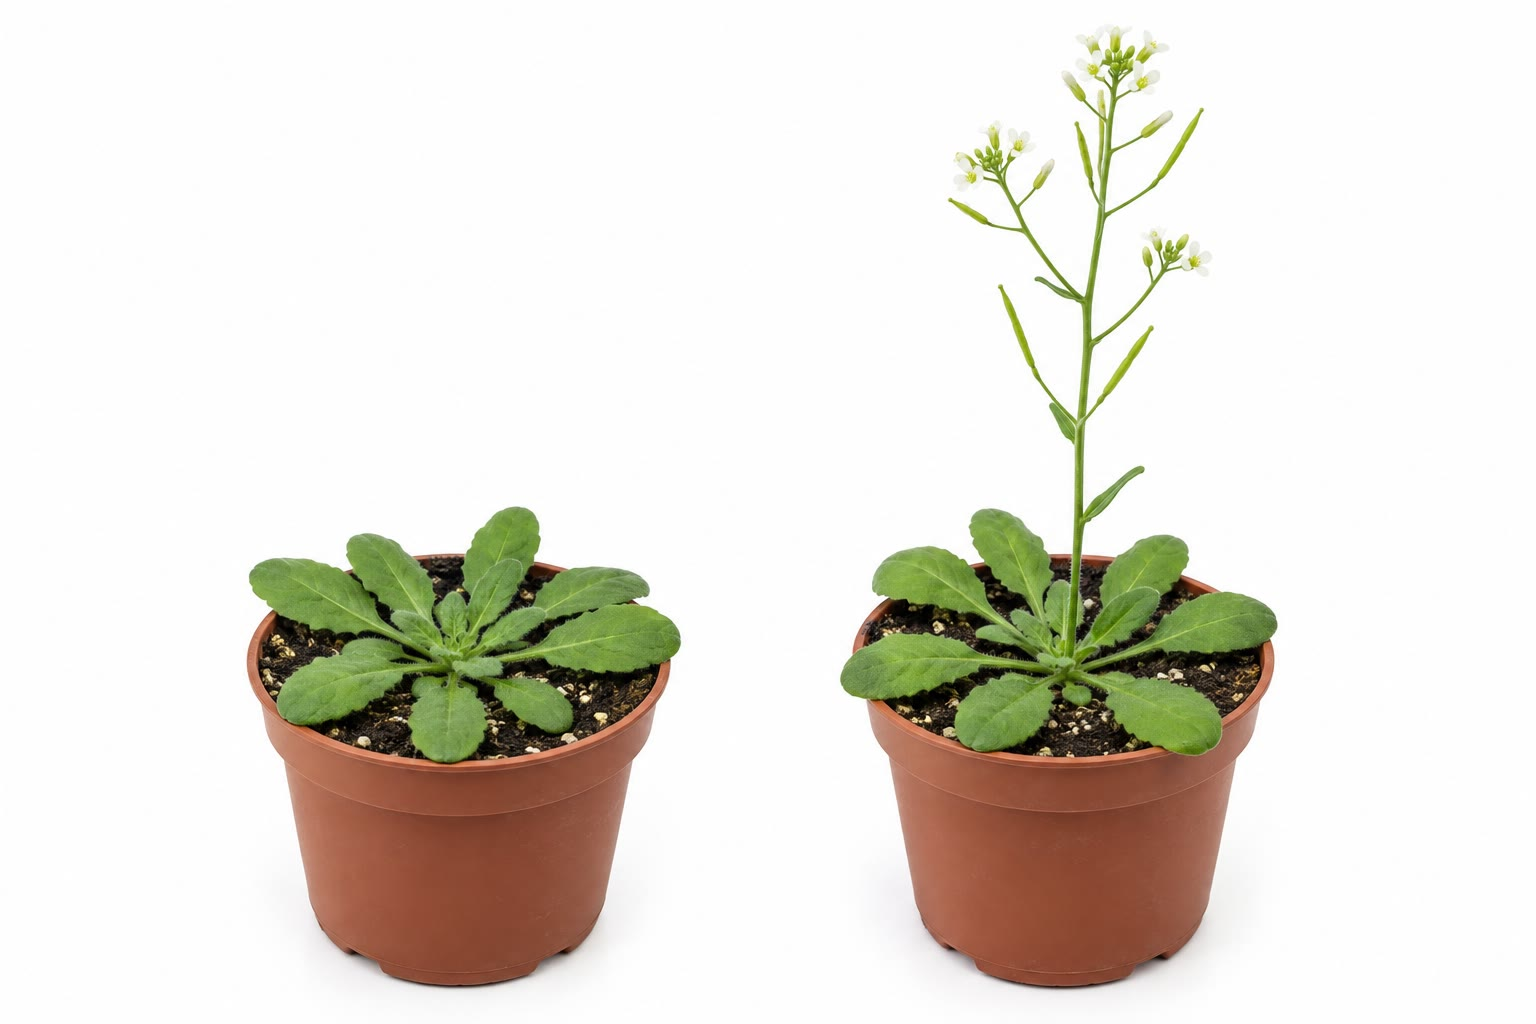
\includegraphics[width=0.58\linewidth]{images/book4/ai/b4-14-arabidopsis-daylength.jpg}

{\small \emph{Arabidopsis}, sebuah \omterm{prop:b2:plant-flowering:photoperiod}{tumbuhan hari panjang}: pada hari
pendek ia berupa sebuah roset daun; dipindahkan ke hari panjang, ia
memanjang lalu berbunga dalam beberapa pekan.}
\end{omfigure}

\begin{proposition}[Vernalisasi: tumbuhannya mencacah dinginnya]\label{prop:b2:plant-flowering:vernalisation}
\index{vernalisasi}\index{FLOWERING LOCUS C}
Serealia musim dingin, tumbuhan dua tahunan (wortel, kubis, digitalis),
dan banyak tumbuhan tahunan iklim dingin tidak akan berbunga sampai
mereka mengalami berpekan-pekan dingin --- yaitu \emph{vernalisasi} ---
yang memastikan bahwa tumbuhan yang berkecambah pada musim gugur
menunggu musim semi alih-alih berbunga ke dalam embun bekunya.
Dinginnya diindera \omterm{def:b2:plant-meristems:meristem}{meristemnya} sendiri, bukan daunnya; ia tidak dapat
digantikan perlakuan lain mana pun; dan pengaruhnya diingat sepanjang
sisa pertumbuhan tumbuhannya, melewati ratusan pembelahan sel, tetapi
tidak melewati \omterm{def:b2:meiosis-heredity:meiosis}{meiosis} --- tiap \omterm{def:b2:angiosperm-reproduction:seed}{biji} bermula tanpa vernalisasi. Pada
\emph{Arabidopsis}, ingatannya adalah sebuah gen, \emph{\omterm{prop:b2:plant-flowering:vernalisation}{FLOWERING LOCUS
C}} (FLC), yang hasilnya menekan pembungaan: berpekan-pekan dingin
membungkamnya secara berangsur dengan menutupi kromatinnya dengan tanda
penekan, pembungamannya disalin pada tiap pembelahannya, dan ia
dihapuskan di dalam lembaganya. Maka tumbuhannya
\emph{mengintegralkan} dinginnya sepanjang waktu --- beberapa hari
dingin tidak berarti --- dan sebuah mutan yang tidak memiliki FLC tidak
membutuhkan musim dingin.
\end{proposition}

\begin{theorem}[Mengapa pengintegralan melindungi dari musim semi palsu]\label{thm:b2:plant-flowering:integration}
Andaikan sebuah penekan dibungkam pada laju tetap $\alpha$ tiap hari
dingin, sehingga sesudah $n$ hari dingin bagian yang masih aktif adalah
$f_n = e^{-\alpha n}$, dan pembungaannya diizinkan ketika $f < f_c$.
Cacah hari dingin yang dibutuhkan adalah $n_c = \ln(1/f_c)/\alpha$, dan
--- karena pembungamannya mantap --- hari dinginnya tidak perlu
berturut-turut: yang berarti adalah jumlahnya. Sebatang tumbuhan dengan
$n_c = 40$ hari tidak tertipu oleh dua pekan pencairan pada bulan
Januari maupun oleh sentakan dingin pada bulan Oktober; tumbuhan yang
hanya mengindera suhu saat ini akan berbunga pada pekan hangat yang
pertama. Pengintegralan yang sama, dengan sebuah ambang, adalah cara
tumbuhannya membaca panjang hari yang tertimbun sebelum memancangkan
diri; keduanya adalah contoh sebuah sistem yang menanggapi
\emph{integral} sebuah isyarat alih-alih nilai seketikanya.
\end{theorem}
\begin{proof}
Kalau tiap hari dinginnya membungkam sebagian $\alpha$ dari salinan
aktif yang tersisa (atau dari kromatin yang masih tak tertandai), bagian
aktifnya memenuhi $f_{n+1} = (1 - \alpha)f_n \approx e^{-\alpha}f_n$,
sehingga $f_n = e^{-\alpha n}$ dengan $n$ sebagai cacah hari dinginnya;
pertidaksamaan $e^{-\alpha n} < f_c$ memberi $n > \ln(1/f_c)/\alpha$.
Hari yang tidak dingin tidak menambah maupun mengurangi, karena
tandanya mantap, sehingga hanya jumlahnya yang berarti.
\end{proof}

\section{Membangun bunganya: model ABC}

\begin{proposition}[Model ABC]\label{prop:b2:plant-flowering:abc}
\index{model ABC}\index{gen homeotik!bunga}
Sebuah \omterm{def:b2:plant-meristems:meristem}{meristem} \omterm{def:b2:angiosperm-reproduction:flower}{bunga} meletakkan empat karangan sepusat: daun kelopak,
daun mahkota, \omterm{def:b2:angiosperm-reproduction:flower}{benang sari}, \omterm{def:b2:angiosperm-reproduction:flower}{daun buah}. Jati dirinya ditetapkan tiga
golongan \emph{gen homeotik}, yang bekerja dalam cincin yang bertindih:
golongan A saja pada karangan 1 memberi daun kelopak; A dan B
bersama-sama pada karangan 2 memberi daun mahkota; B dan C bersama-sama
pada karangan 3 memberi \omterm{def:b2:angiosperm-reproduction:flower}{benang sari}; C saja pada karangan 4 memberi
\omterm{def:b2:angiosperm-reproduction:flower}{daun buah}. A dan C saling menekan, sehingga di tempat salah satunya
hilang, yang lain menyebar ke seluruh \omterm{def:b2:angiosperm-reproduction:flower}{bunganya}. Kaidahnya meramalkan
tiap mutan tunggalnya: hilangkan B dan \omterm{def:b2:angiosperm-reproduction:flower}{bunganya} menjadi kelopak--kelopak--
daun buah--daun \omterm{def:b2:angiosperm-reproduction:seed}{buah}; hilangkan C dan ia menjadi
kelopak--mahkota--mahkota--kelopak, lalu sekuntum \omterm{def:b2:angiosperm-reproduction:flower}{bunga} lagi di
dalamnya, karena C juga menghentikan \omterm{def:b2:plant-meristems:meristem}{meristemnya}; hilangkan A dan ia
menjadi daun buah--benang sari--benang sari--daun \omterm{def:b2:angiosperm-reproduction:seed}{buah}. Sebagian besar
gen ini menyandikan \omterm{prop:b2:cell-differentiation:transcriptional}{faktor transkripsi} satu keluarga (kotak MADS), dan
golongan keempat, yaitu E, dibutuhkan bagi ketiga fungsinya;
mengungkapkan B dan C bersama-sama di dalam sehelai daun mengubahnya
menjadi organ mirip \omterm{def:b2:angiosperm-reproduction:flower}{benang sari}. \omterm{def:b2:angiosperm-reproduction:flower}{Bunga} ganda di taman --- mawar, peoni,
kamelia --- adalah mutan golongan C, yang \omterm{def:b2:angiosperm-reproduction:flower}{benang sarinya} berubah
menjadi daun mahkota tambahan.
\end{proposition}
\begin{proof}[Bukti eksperimental]
Coen dan Meyerowitz (1991) membandingkan mutan homeotik
\emph{Arabidopsis} dan snapdragon: pada keduanya, tiga golongan \omterm{def:b2:genome-diversification:mutation}{mutasi}
masing-masing mengubah dua karangan yang bersebelahan, dalam pasangan
yang sama, dan gabungan mutannya berperilaku seperti yang diramalkan
modelnya (mutan rangkap tiganya hanya membuat daun). Pengklonaan
menunjukkan gennya sebagai \omterm{prop:b2:cell-differentiation:transcriptional}{faktor transkripsi} yang diungkapkan dalam
cincin yang diramalkan; menaruh sebuah gen B di bawah sebuah promotor
yang aktif pada keempat karangannya memberi
mahkota--mahkota--benang sari--benang sari.
\end{proof}

\begin{omfigure}
\begin{tikzpicture}[every node/.style={font=\scriptsize}]
  % four whorls as columns
  \foreach \x/\w in {0/{karangan 1}, 2.2/{karangan 2}, 4.4/{karangan 3}, 6.6/{karangan 4}} \node[above] at (\x+0.9,3.3) {\w};
  \fill[omDef!35] (0,2.4) rectangle (4.2,3.1); \node at (2.1,2.75) {A};
  \fill[omProp!40] (2.2,1.6) rectangle (6.4,2.3); \node at (4.3,1.95) {B};
  \fill[omThm!30] (4.4,0.8) rectangle (8.6,1.5); \node at (6.5,1.15) {C};
  \foreach \x/\o in {0/{daun kelopak}, 2.2/{daun mahkota}, 4.4/{benang sari}, 6.6/{daun buah}} \node[below, align=center] at (\x+0.9,0.6) {\o};
  \node[anchor=west, align=left] at (9.2,3.0) {tipe liar: A, AB, BC, C};
  \node[anchor=west, align=left] at (9.2,2.3) {tanpa B: kelopak, kelopak, buah, buah};
  \node[anchor=west, align=left] at (9.2,1.6) {tanpa C: kelopak, mahkota, mahkota, kelopak\ldots};
  \node[anchor=west, align=left] at (9.2,0.9) {tanpa A: buah, sari, sari, buah};
\end{tikzpicture}

{\small \omterm{prop:b2:plant-flowering:abc}{Model ABC}. Tiga golongan gen dalam cincin yang bertindih
menetapkan keempat jati diri organnya; kehilangan satu golongan
mengubah dua karangan, dan \omterm{def:b2:angiosperm-reproduction:flower}{bunga} mutannya persis seperti yang
diramalkan.}
\end{omfigure}

\begin{omfigure}
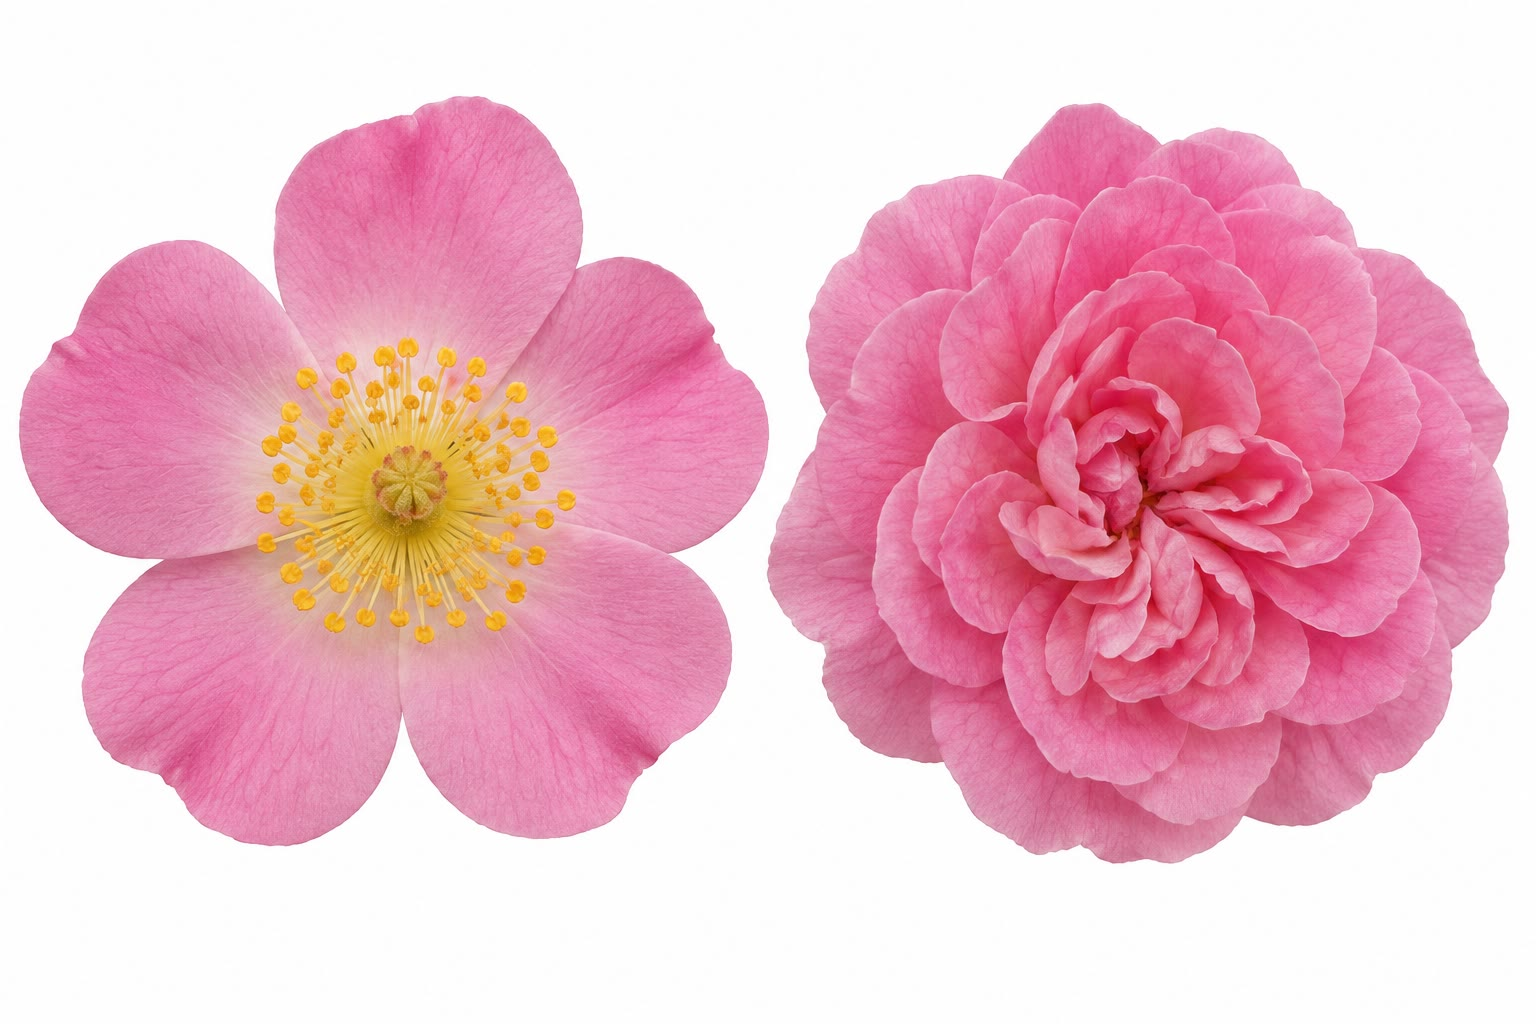
\includegraphics[width=0.58\linewidth]{images/book4/ai/b4-14-double-flower.jpg}

{\small Sekuntum \omterm{def:b2:angiosperm-reproduction:flower}{bunga} tipe liar di samping sebuah bentuk ganda: \omterm{def:b2:angiosperm-reproduction:flower}{benang
sarinya} telah menjadi daun mahkota --- sebuah mutan golongan C, yang
dipilih tukang kebun berabad-abad sebelum ada yang tahu mengapa ia
ganda.}
\end{omfigure}

\section{Dormansi dan perkecambahan}

\begin{definition}[Dormansi biji]\label{def:b2:plant-flowering:dormancy}
\index{dormansi!biji}\index{asam absisat}\index{giberelin}\index{stratifikasi}
Sebutir \omterm{def:b2:angiosperm-reproduction:seed}{biji} yang hidup tetapi tidak berkecambah dalam keadaan yang
sesungguhnya menyokong pertumbuhan disebut \emph{dorman}. \omterm{def:b2:angiosperm-reproduction:seed}{Dormansinya}
dipaksakan selama pemasakan \omterm{def:b2:angiosperm-reproduction:seed}{bijinya} oleh \emph{asam absisat} (ABA),
yang juga menggerakkan penimbunan cadangannya dan pengeringan
lembaganya, dan ia dipertahankan \omterm{def:b2:angiosperm-reproduction:seed}{kulit bijinya} (tak tertembus air atau
oksigen, dan menahan secara mekanik) atau oleh keadaan lembaganya
sendiri. Ia dipatahkan isyarat yang menandai akhir musim yang tidak
menguntungkan: berpekan-pekan dingin dan lembap (\emph{stratifikasi},
yaitu vernalisasi \omterm{def:b2:angiosperm-reproduction:seed}{bijinya}), cahaya --- bagi \omterm{def:b2:angiosperm-reproduction:seed}{biji} kecil yang harus
berada dekat permukaannya, yang diindera fitokrom --- atau kegelapan,
suhu yang berganti-ganti, pelucutan penghambatnya oleh hujan,
penggoresan kulitnya oleh tanah atau sebuah usus, asap dan bahang
sesudah kebakaran. Keputusannya adalah sebuah keseimbangan antara ABA
dan \emph{giberelin}: isyarat pemecahnya menurunkan ABA dan menaikkan
giberelin, yang membangkitkan cadangannya
(\cref{ch:b2:angiosperm-reproduction}) lalu membiarkan radikelnya
tumbuh. Sebuah populasi \omterm{def:b2:angiosperm-reproduction:seed}{biji} tidaklah seragam: sebagian berkecambah
pada kesempatan pertamanya, sisanya menunggu setahun atau lebih,
sehingga tidak ada satu musim buruk pun yang membunuh seluruh
kelompoknya --- itulah \emph{lumbung \omterm{def:b2:angiosperm-reproduction:seed}{biji}}, sebuah lindungan terhadap
dunia yang tak teramalkan.
\end{definition}
\begin{proof}[Bukti eksperimental]
\omterm{def:b2:angiosperm-reproduction:seed}{Biji} selada (Borthwick, 1952) berkecambah di dalam gelap sesudah
sekilas cahaya merah dan tidak sesudah sekilas merah-jauh; diberi merah
lalu merah-jauh lalu merah, mereka berkecambah --- kilasan terakhirnya
yang memutuskan. Pigmen terbalikkan yang sama yang mewaktui
pembungaannya memulai perkecambahannya. \omterm{def:b2:angiosperm-reproduction:seed}{Biji} banyak pohon yang ditanam
segar di tanah yang hangat tidak melakukan apa pun; \omterm{def:b2:angiosperm-reproduction:seed}{biji} yang sama
sesudah dua bulan di dalam lemari es yang lembap berkecambah seketika,
dan mutan yang kekurangan ABA berkecambah di atas tumbuhannya bahkan
sebelum \omterm{def:b2:angiosperm-reproduction:seed}{bijinya} kering.
\end{proof}

\begin{omfigure}
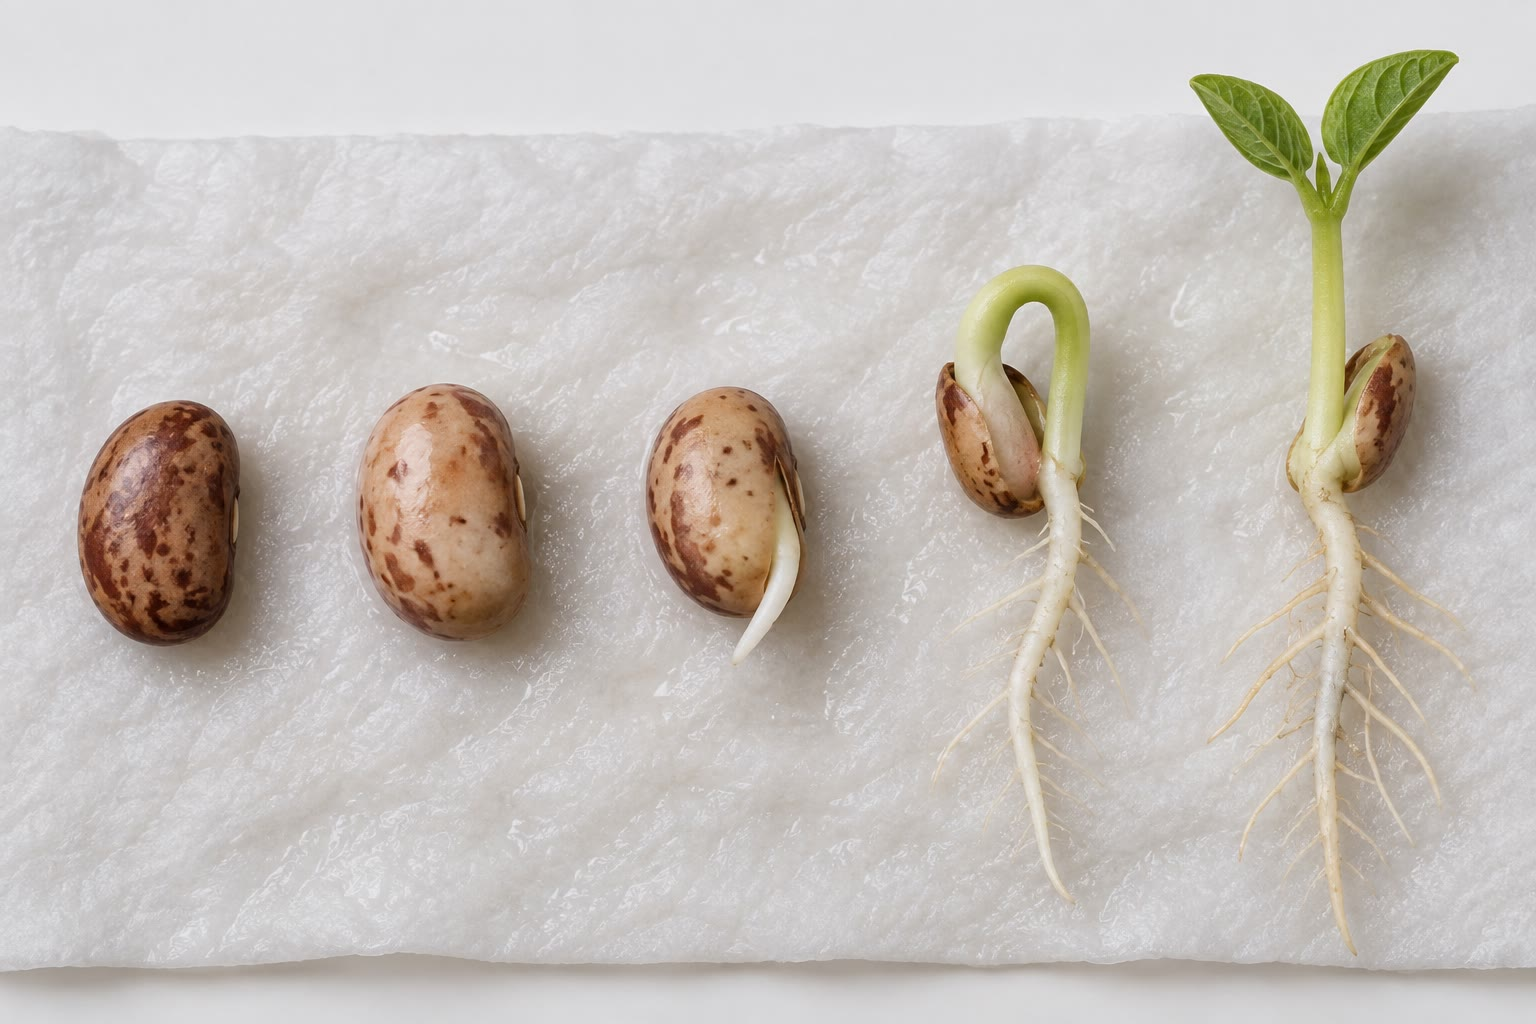
\includegraphics[width=0.66\linewidth]{images/book4/ai/b4-14-germinating-beans.jpg}

{\small Perkecambahan buncis: \omterm{def:b2:angiosperm-reproduction:seed}{bijinya} mengimbibisi air, radikelnya
muncul lebih dahulu, hipokotilnya mengait ke atas menembus tanahnya,
dan kaitnya meluruskan diri di dalam cahaya sembari daun pertamanya
membuka.}
\end{omfigure}

\begin{theorem}[Perkecambahan sebagai sebuah taruhan]\label{thm:b2:plant-flowering:bet}
\index{pelindungan taruhan}
Misalkan sebagian $g$ dari sekelompok \omterm{def:b2:angiosperm-reproduction:seed}{biji} berkecambah tiap tahun dan
sisanya bertahan hidup di dalam tanahnya dengan peluang $s$ sampai
tahun berikutnya. Pada tahun yang baik, sebutir \omterm{def:b2:angiosperm-reproduction:seed}{biji} yang berkecambah
meninggalkan $R_g$ \omterm{def:b2:angiosperm-reproduction:seed}{biji}; pada tahun yang buruk, tidak satu pun;
tahunnya baik dengan peluang $p$. Sebuah siasat yang mengecambahkan
segalanya sekaligus ($g = 1$) memiliki, sepanjang serangkaian tahun,
laju pertumbuhan jangka panjang yang dipurata secara $\ln$ sebagai
$p\ln R_g + (1 - p)\ln 0 =
-\infty$: satu tahun yang buruk
memusnahkannya. Sebuah siasat dengan $g < 1$ tumbuh pada tahun yang
baik dengan faktor $gR_g + (1 - g)s$ dan pada tahun yang buruk dengan
$(1 - g)s > 0$, sehingga laju jangka panjangnya,
\[
r = p\ln\bigl(gR_g + (1 - g)s\bigr) + (1 - p)\ln\bigl((1 - g)s\bigr),
\]
berhingga dan, bagi $p$ yang tidak terlalu dekat dengan 1, mencapai
maksimumnya pada $g$ yang di tengah. Dengan $R_g = 20$, $s = 0.8$, dan
$p = 0.7$, optimumnya di dekat $g = 0.7$: kecambahkan sebagian besarnya,
simpan sebuah cadangan. \omterm{def:b2:angiosperm-reproduction:seed}{Dormansi} bukanlah kegagalan berkecambah
melainkan penolakan sebagian yang telah berkembang.
\end{theorem}
\begin{proof}
Ukuran populasinya sesudah $T$ tahun adalah hasil kali faktor
tahunannya, sehingga laju pertumbuhannya adalah purata logaritmanya
(yaitu laju purata geometrik), dan itulah yang dimaksimumkan seleksi
sepanjang rentang yang panjang. Dengan $g = 1$, faktor tahun buruknya
nol dan logaritmanya $-\infty$. Bagi $g < 1$ kedua faktornya positif;
mendiferensialkan $r$ terhadap $g$ lalu menetapkan turunannya nol
memberi optimumnya, yang bagi angka yang dikutip terletak di dekat
$g = 0.7$ (menghitung $r$ pada $g = 0.4, 0.6, 0.8, 1$ memberi $1.28$,
$1.42$, $1.40$, $-\infty$).
\end{proof}

\begin{omfigure}
\begin{tikzpicture}
\begin{axis}[
  width=0.7\linewidth, height=5.4cm,
  axis x line=bottom, axis y line=left,
  xmin=0, xmax=1, ymin=0, ymax=1.7,
  xlabel={bagian yang berkecambah tiap tahun, $g$}, ylabel={laju pertumbuhan jangka panjang $r$},
  xlabel style={font=\small, at={(axis description cs:0.5,-0.13)}, anchor=north},
  ylabel style={font=\small},
  tick label style={font=\small}, xtick={0,0.2,0.4,0.6,0.8,1}, ytick={0,0.5,1,1.5},
  clip=false,
]
\addplot[very thick, omDef, domain=0.02:0.97, samples=100] {0.7*ln(20*x + 0.8*(1-x)) + 0.3*ln(0.8*(1-x))};
\draw[dashed, gray] (axis cs:0.7,0) -- (axis cs:0.7,1.43);
\node[font=\scriptsize, anchor=south] at (axis cs:0.7,1.45) {optimum: simpan \qty{30}{\%} di dalam tanahnya};
\node[font=\scriptsize, anchor=north west, align=left] at (axis cs:0.7,0.6) {$g \to 1$: satu tahun buruk\\memusnahkan kelompoknya};
\end{axis}
\end{tikzpicture}

{\small \omterm{thm:b2:plant-flowering:bet}{Pelindungan taruhan} lewat \omterm{def:b2:angiosperm-reproduction:seed}{dormansi}. Dengan tahun yang baik
tujuh kali dari sepuluh, sekelompok \omterm{def:b2:angiosperm-reproduction:seed}{biji} yang berkecambah seluruhnya
akhirnya dimusnahkan sebuah tahun yang buruk; sekelompok \omterm{def:b2:angiosperm-reproduction:seed}{biji} yang
menahan sebagian \omterm{def:b2:angiosperm-reproduction:seed}{bijinya} tumbuh paling cepat dalam jangka panjang.}
\end{omfigure}

\section{Latihan}

\begin{exercise}[$\star$]\label{exo:b2:plant-flowering:1}
Bedakanlah \omterm{def:b2:plant-meristems:meristem}{meristem} vegetatif, \omterm{def:b2:plant-flowering:transition}{meristem perbungaan}, dan \omterm{def:b2:plant-meristems:meristem}{meristem} \omterm{def:b2:angiosperm-reproduction:flower}{bunga},
lalu katakan mana yang bersifat tertentu.
\end{exercise}

\begin{exercise}[$\star$]\label{exo:b2:plant-flowering:2}
Definisikan \omterm{prop:b2:plant-flowering:photoperiod}{tumbuhan hari pendek}, hari panjang, dan netral hari beserta
sebuah contoh masing-masingnya, lalu katakan apa yang sesungguhnya
diukur sebuah \omterm{prop:b2:plant-flowering:photoperiod}{tumbuhan hari pendek}.
\end{exercise}

\begin{exercise}[$\star$]\label{exo:b2:plant-flowering:3}
Berikan jati diri organ tiap karangannya pada tipe liarnya dan pada
ketiga mutan tunggal \omterm{prop:b2:plant-flowering:abc}{model ABC}.
\end{exercise}

\begin{exercise}[$\star$]\label{exo:b2:plant-flowering:4}
Sebutkan empat isyarat yang mematahkan \omterm{def:b2:angiosperm-reproduction:seed}{dormansi} \omterm{def:b2:angiosperm-reproduction:seed}{biji} dan, bagi
masing-masingnya, musim atau tempat yang dilaporkannya.
\end{exercise}

\begin{exercise}[$\star\star$]\label{exo:b2:plant-flowering:5}
Sebuah \omterm{prop:b2:plant-flowering:photoperiod}{tumbuhan hari pendek} memiliki malam kritis \qty{10}{h}.
Katakanlah apakah ia berbunga di bawah: \qty{16}{h} terang/\qty{8}{h} gelap;
\qty{12}{h}/\qty{12}{h}; \qty{12}{h} terang, \qty{6}{h} gelap, semenit
cahaya, \qty{6}{h} gelap; \qty{8}{h} terang, \qty{4}{h} gelap,
\qty{4}{h} terang, \qty{8}{h} gelap.
\end{exercise}

\begin{exercise}[$\star\star$]\label{exo:b2:plant-flowering:6}
Sehelai daun sebuah \omterm{prop:b2:plant-flowering:photoperiod}{tumbuhan hari pendek} yang terimbas dicangkokkan
pada sebuah \omterm{prop:b2:plant-flowering:photoperiod}{tumbuhan hari panjang} yang dijaga pada hari panjang, dan
\omterm{prop:b2:plant-flowering:photoperiod}{tumbuhan hari panjangnya} berbunga. Apa yang ditunjukkannya tentang
\omterm{def:b2:plant-flowering:florigen}{florigen}? Bagaimana kalau cangkokannya dibuat dengan sehelai daun yang
telah terimbas tetapi floemnya diputus pada tangkai daunnya?
\end{exercise}

\begin{exercise}[$\star\star$]\label{exo:b2:plant-flowering:7}
Dingin membungkam penekannya pada $\alpha = 0.05$ tiap hari dan
pembungaannya menuntut $f < 0.15$. Berapa hari dingin yang dibutuhkan?
Sebuah musim dingin memiliki tiga giliran dingin selama 15, 12, dan 20
hari yang dipisahkan pencairan: apakah tumbuhannya tervernalisasi?
Bagaimana kalau $\alpha$-nya $0.02$?
\end{exercise}

\begin{exercise}[$\star\star$]\label{exo:b2:plant-flowering:8}
Jelaskan mengapa ingatan sebatang tumbuhan yang tervernalisasi hilang
di dalam \omterm{def:b2:angiosperm-reproduction:seed}{bijinya}, dari segi kromatinnya, dan mengapa hal itu berguna.
\end{exercise}

\begin{exercise}[$\star\star$]\label{exo:b2:plant-flowering:9}
\omterm{def:b2:angiosperm-reproduction:seed}{Biji} selada diberi, di dalam gelap, urutan: M; M lalu MJ; M, MJ, M;
M, MJ, M, MJ. Ramalkanlah perkecambahannya pada tiap kasusnya lalu
jelaskan dari segi kedua bentuk fitokromnya.
\end{exercise}

\begin{exercise}[$\star\star\star$]\label{exo:b2:plant-flowering:10}
Pada model \omterm{thm:b2:plant-flowering:bet}{pelindungan taruhannya} dengan $R_g = 20$, $s = 0.8$,
hitunglah laju pertumbuhan jangka panjangnya bagi $g = 0.4$, $0.6$,
$0.8$, dan $1$ ketika $p = 0.7$, lalu sekali lagi ketika $p = 0.95$.
Bagaimana optimumnya bergeser, dan apa yang diramalkannya bagi gurun
dibandingkan padang rumput?
\end{exercise}

\begin{exercise}[$\star\star\star$]\label{exo:b2:plant-flowering:11}
Ramalkanlah \omterm{def:b2:angiosperm-reproduction:flower}{bunga} yang dihasilkan dengan mengungkapkan sebuah gen
golongan B pada keempat karangannya; dengan mengungkapkan golongan C
pada keempatnya; dan oleh sebuah mutan ganda yang tidak memiliki A
maupun B. Lalu jelaskan mengapa \omterm{def:b2:angiosperm-reproduction:flower}{bunga} tanpa C terus membuat karangan.
\end{exercise}

\begin{exercise}[$\star\star\star$]\label{exo:b2:plant-flowering:12}
``Sebatang tumbuhan memutuskan untuk berbunga dengan mengintegralkan
isyarat yang tidak dapat dikendalikannya.'' Bahaslah ketiga
pengintegralan bab ini --- panjang harinya, dinginnya, dan tahun di
dalam lumbung \omterm{def:b2:angiosperm-reproduction:seed}{bijinya} --- serta apa yang dilindungi sebuah pengintegral
bagi tumbuhannya yang tidak dilindungi sebuah ambang sederhana.
\end{exercise}

\section{Soal: Kalender Sang Penanam}

\begin{problem}[{Soal akhir pekan --- seorang penanam krisan menjadwalkan
pembungaan dengan lampu, seorang pemulia gandum mencacah dingin, bunga
ganda seorang perangkai bunga dijelaskan, dan dormansi sekelompok biji
dimodelkan, berakhir pada panjang malam yang memicu panennya, hari
dingin yang dibutuhkan gandumnya, dan bagian perkecambahan terbaiknya}]
\label{pb:b2:plant-flowering:1}
Krisan adalah \omterm{prop:b2:plant-flowering:photoperiod}{tumbuhan hari pendek} dengan panjang malam kritis
\qty{9.5}{h}; pengimbasannya menuntut \num{12} malam pengimbas
berturut-turut, dan \omterm{def:b2:angiosperm-reproduction:flower}{bunganya} membuka \num{8} pekan sesudah
pengimbasannya. Pada bulan November rumah kacanya gelap dari pukul
17.00 sampai 07.30. Gandum musim dingin memiliki $\alpha = 0.06$ tiap
hari dingin dan berbunga ketika $f < 0.10$. Kelompok \omterm{def:b2:angiosperm-reproduction:seed}{bijinya}:
$R_g = 15$, $s = 0.7$, tahun baik dengan peluang $p$.

\medskip
\noindent\textbf{Bagian I --- Rumah kacanya.}
\begin{enumerate}
  \item Pada bulan Juni malam alaminya \qty{8}{h}. Akankah panennya
        berbunga? Apa yang harus dikerjakan penanamnya agar dapat
        menjual \omterm{def:b2:angiosperm-reproduction:flower}{bunga} pada bulan Agustus?
  \item Penanamnya menutupi panennya dengan kain hitam dari pukul
        19.00 sampai 07.00. Panjang malam berapa yang dilihat
        tumbuhannya, dan kapan penutupannya harus mulai agar \omterm{def:b2:angiosperm-reproduction:flower}{bunganya}
        membuka pada 15~Agustus?
  \item Pada bulan November malam alaminya \qty{14}{h} dan penanamnya
        ingin \emph{menunda} pembungaannya sampai Natal. Usulkanlah
        sebuah jadwal penyinaran lalu jelaskan mengapa sekilas cahaya
        sudah mencukupi.
  \item Kilasannya diberikan pada pukul 21.00 alih-alih pada pukul
        00.00, dan pengimbasannya tidak tercegah. Jelaskan dengan
        panjang malam kritisnya.
  \item Satu malam dari kedua belasnya, kainnya tertinggal terbuka.
        Ramalkanlah, lalu katakan apa yang akan dikerjakan sebatang
        kokelbur.
  \item Kilasannya diberikan dalam cahaya hijau dan gagal; dalam
        cahaya merah ia berhasil; merah yang diikuti merah-jauh gagal.
        Jelaskan.
  \item Sehelai daun sebatang tumbuhan yang terimbas dicangkokkan pada
        sebatang tumbuhan di bawah hari panjang. Ramalkanlah, lalu
        katakan apa yang dikenalinya.
\end{enumerate}

\medskip
\noindent\textbf{Bagian II --- Gandumnya.}
\begin{enumerate}[resume]
  \item Berapa hari dingin yang dibutuhkan gandumnya?
  \item Ditanam pada bulan Oktober, ia memperoleh 10 hari dingin pada
        bulan November, sebuah Desember yang sejuk, 25 hari pada bulan
        Januari, dan 12 hari pada bulan Februari. Kapan ia
        tervernalisasi?
  \item Ditanam pada bulan Maret, ia memperoleh 6 hari dingin. Apakah
        ia berbunga pada musim panas itu? Apa akibatnya bagi
        pertaniannya?
  \item Sebuah mutan tidak memiliki penekannya. Ramalkanlah
        perilakunya lalu katakan mengapa pemulia menyebut gandum
        semacam itu ``gandum musim semi''.
  \item Jelaskan mengapa ingatan dinginnya selamat dari pembelahan
        \omterm{def:b2:plant-meristems:meristem}{meristemnya} sepanjang musim semi tetapi tidak dari \omterm{def:b2:meiosis-heredity:meiosis}{meiosis} yang
        membuat generasi berikutnya.
  \item Mengapa dinginnya harus dicacah di dalam \omterm{def:b2:plant-meristems:meristem}{meristemnya} dan tidak
        di dalam daunnya, tidak seperti panjang harinya?
\end{enumerate}

\medskip
\noindent\textbf{Bagian III --- Perangkai \omterm{def:b2:angiosperm-reproduction:flower}{bunganya}.}
\begin{enumerate}[resume]
  \item Sebuah mawar ganda memiliki daun mahkota di tempat \omterm{def:b2:angiosperm-reproduction:flower}{benang
        sarinya} seharusnya berada dan beberapa daun mahkota tambahan di
        pusatnya. Golongan gen mana yang gagal? Berikan rumus
        karangannya.
  \item Mawar semacam itu mandul sebagai tetua \omterm{def:b2:plant-life-cycles:heterospory}{serbuk sari} tetapi
        kadang menjadikan \omterm{def:b2:angiosperm-reproduction:seed}{biji}. Jelaskan kedua kenyataannya dari \omterm{prop:b2:plant-flowering:abc}{model
        ABC}.
  \item Sebuah snapdragon memiliki \omterm{def:b2:angiosperm-reproduction:flower}{benang sari} di tempat daun
        mahkotanya dan \omterm{def:b2:angiosperm-reproduction:flower}{daun buah} di tempat daun kelopaknya. Golongan
        mana yang gagal?
  \item Ramalkanlah \omterm{def:b2:angiosperm-reproduction:flower}{bunga} sebatang tumbuhan yang golongan C-nya
        diungkapkan pada karangan 1 selain pada karangan normalnya.
  \item Mengapa \omterm{def:b2:genome-diversification:mutation}{mutasi} yang sama menghasilkan perubahan yang sama pada
        sebuah mawar, sebuah snapdragon, dan \emph{Arabidopsis}, yaitu
        tumbuhan yang terpisah seratus juta tahun?
  \item Pada karangan 2 sekuntum \omterm{def:b2:angiosperm-reproduction:flower}{bunga} tipe liar, A dan B sama-sama
        aktif. Ramalkanlah organnya kalau hanya B yang aktif di situ.
\end{enumerate}

\medskip
\noindent\textbf{Bagian IV --- Kelompok \omterm{def:b2:angiosperm-reproduction:seed}{bijinya}.}
\begin{enumerate}[resume]
  \item Hitunglah laju pertumbuhan jangka panjang $r$ bagi $g = 0.5$,
        $0.7$, dan $0.9$ ketika $p = 0.8$.
  \item Mana di antara ketiganya yang terbaik? Apa yang terjadi pada
        $g = 1$?
  \item Hitunglah kembali bagi $p = 0.5$ (sebuah gurun). $g$ mana yang
        terbaik sekarang?
  \item Seorang penanam menanam seluruh kelompoknya di satu ladang
        pada tahun yang baik lalu memanen $R_g$ tiap \omterm{def:b2:angiosperm-reproduction:seed}{bijinya}. Jelaskan
        mengapa siasatnya berbeda dari siasat tumbuhannya dan apa yang
        harus dikerjakannya untuk mempertahankan varietasnya melewati
        sebuah tahun yang buruk.
  \item \omterm{def:b2:angiosperm-reproduction:seed}{Bijinya} membutuhkan cahaya untuk berkecambah. Jelaskan makna
        adaptif hal ini bagi sebutir \omterm{def:b2:angiosperm-reproduction:seed}{biji} yang kecil, lalu ramalkan apa
        yang dikerjakan pembajakan pada lumbung \omterm{def:b2:angiosperm-reproduction:seed}{bijinya}.
  \item Nyatakan hasilnya: panjang malam kritisnya dan jadwal
        penutupannya, kebutuhan dingin gandumnya, serta $g$ terbaik
        bagi $p = 0.8$ dan $p = 0.5$.
\end{enumerate}
\end{problem}
